\section{Results and Discussion}\label{sec:result}
{\color{red}{SS: Any need to list the number of steps we take to generate final model?}}

The step of shape optimization in our paper can be best demonstrated on the model~\ref{fig:result}, through initialization, we can have a rough concept of the final model, and by user interaction including selecting vertices merged and faces in the same plane, we can finally generate a pleasing model from a given structural layout.

We show a number of 3D models generated by our system Figure~\ref{fig:more}, and most of the cases can have an ideal result after initialization because of the cuboid shape as Figure~\ref{fig:more} (a). Through interaction, users can folding more complicated cartons to ideal shapes as Figure~\ref{fig:more} (b).

However, the initialization will not generate a pleasing result on some complicated cases, and leads to the difficult interaction to get the final model. As for Figure~\ref{fig:limitation}, to have a better corresponding model, users need to take at least ten steps to get to Figure~\ref{fig:limitation}(c). 


\begin{figure}
	\centering
	\includegraphics[width=0.9\textwidth]{images/result.jpg}
	\caption{Structural layout (a) is used to generate flat polymesh (b), and then initialize to a rough model (c), after merge the three vertices in red circles (c) and the two vertices circled red (d), the model is almost closed with two paste faces in red and pink outside the carton (e), finally through selecting these faces are in the same plane of the yellow face as surface, we can have the final model (f).}
	\label{fig:result}
\end{figure}

\begin{figure}
	\centering
	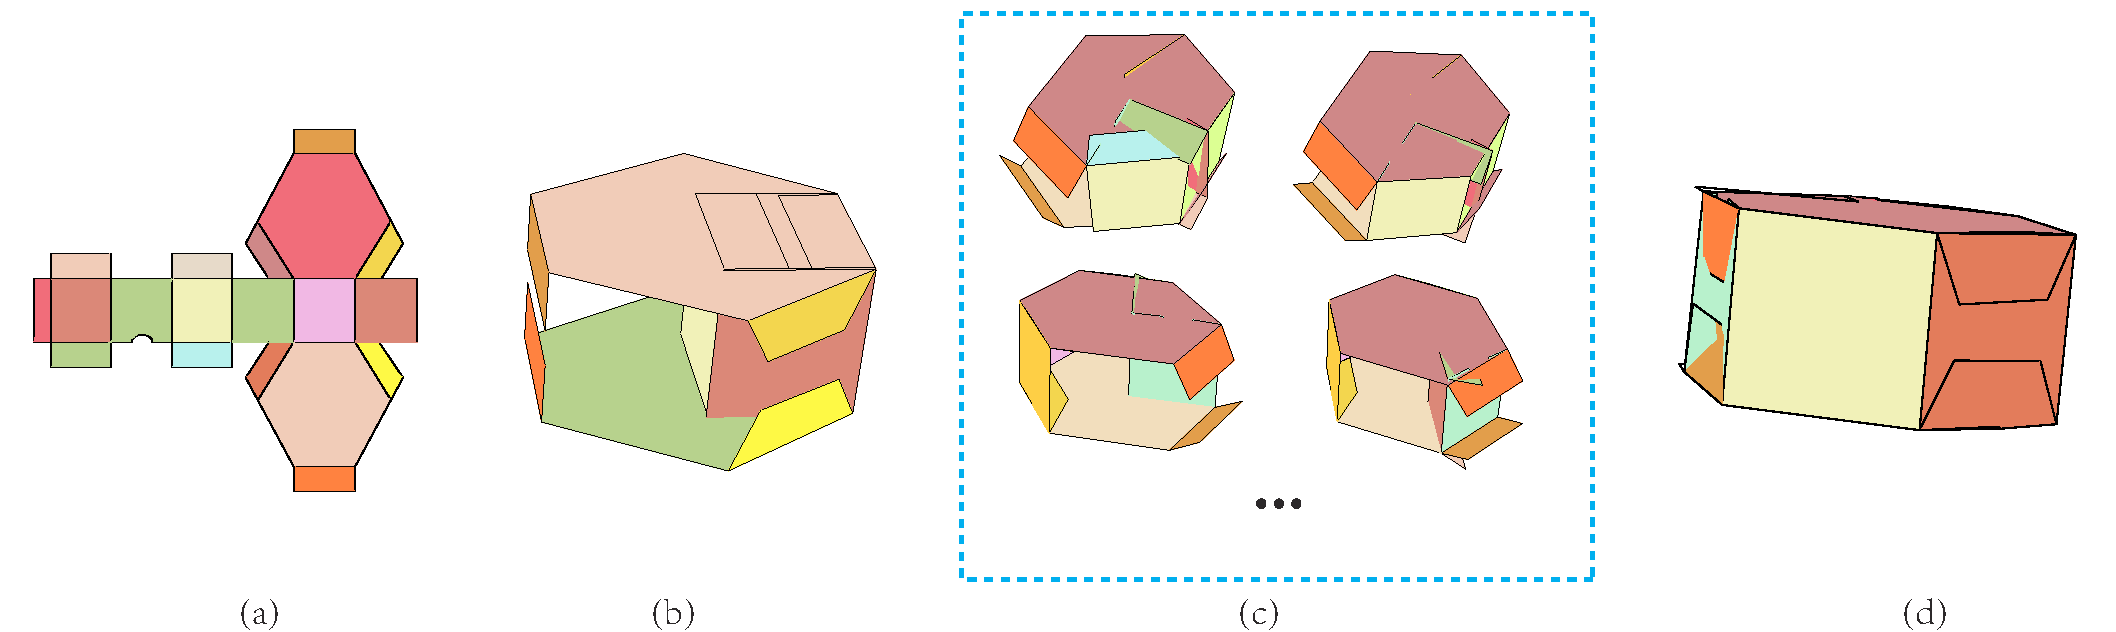
\includegraphics[width=0.9\textwidth]{images/limitation.jpg}
	\caption{Given a layout as (a), our system can generate an initialized result as (b), and through at least ten steps including select vertices need to be the same place and faces need to be coplane , users can get the final model as (c).}
	\label{fig:limitation}
\end{figure}

\begin{figure}
	\centering
	\includegraphics[width=0.9\textwidth]{images/more.jpg}
	\caption{More results, part of cartons can be initialized without refining (a), and with interaction, users can manipulate more complicated cartons (b). The first and second column in (a) and (b) are the flat mesh and initialization result of cartons, and the last column in (b) shows the model after interaction.}
	\label{fig:more}
\end{figure}